\documentclass[10pt, letterpaper]{article}
        \usepackage[utf8]{inputenc}
        \usepackage[margin=1in]{geometry}
        \usepackage{fancyhdr}
        \usepackage{titling}
        \usepackage{enumitem}
        \usepackage{mathtools}
        \usepackage{amssymb}
        \usepackage{xfrac}
        \usepackage{booktabs}
        \usepackage{graphicx}
        \usepackage{wrapfig, blindtext}
        \usepackage{hyperref}
        \usepackage{enumerate}
        \usepackage{multicol}

        
        \setlength{\parindent}{0pt}

\title{Journal 2}
        \author{Sudhan Chitgopkar}
        \date{\today}
        
        % headers -- no need to change
        \pagestyle{fancy}
        \fancyhf{}
        \lhead{The Mahabharata}
        \chead{UGAMUNC XXVII}
        \rhead{\thedate}


\begin{document}

Greetings Delegates! \\

On behalf of the University of Georgia, I would like to welcome you to
UGAMUNC XXVIII and the
\texttt{\underline{\href{https://drive.google.com/file/d/12-b_zmhinbKkOyAVeJg0iiA7b07jg8uN/view?usp=sharing}{\textbf{Mahabharata}}}
(mah-haa-baa-ruth)} Committee. My name is Manashi Patel, and I have the
honor of serving as your crisis director for the conference. I am a
senior from Waycross, Georgia studying accounting and political science.
I am a part of Greek life on campus; I'm a member of Alpha Kappa Psi - a
co-ed business fraternity. In my free time, I love to read, hike, or
watch the news or Netflix. Some of my favorite shows to watch are New
Girl, Friends, The Patriot Act, and The Office. I'm really excited to
meet all of you in February! \\

I also have the pleasure of introducing the committee chair,
\texttt{\underline{\href{https://drive.google.com/file/d/1_S9ve7zhbbZEV1lCzaMhAx-Lk6sWg8dz/view?usp=sharing}{\textbf{Namrata}}
(num-ruh-tha)}} Kella \\
(\texttt{\href{mailto:namukella@gmail.com}{\underline{namukella@gmail.com}}}).
She is a third-year International Affairs major and Spanish minor from
Alpharetta, Georgia. Some of her favorite organizations she's involved
in on-campus are Georgia Political Review, SPIA Ambassadors, and of
course, Model UN. In her free time, Namrata enjoys thrifting, cooking,
photography, and drinking iced coffee regardless of the season. \\

This is her 3rd year on the Model UN team and her 2nd year chairing and
she is so thankful for the friends she's made and the skills she's
learned during her time on the team so far. \\

I'm also excited to introduce the co-chair for the committee,
\texttt{\underline{\href{https://drive.google.com/file/d/15s-ZAYrA7ZARL66gJE8hjQ4EltP_k3Q9/view?usp=sharing}{\textbf{Ashni}}
(uhsh-nee)}} Patel
(\texttt{\href{mailto:ashni.patel1@uga.edu}{\underline{ashni.patel1@uga.edu}}}).
She is a first-year majoring in International Affairs with a minor in
Statistics from Sandy Springs, Georgia. She is also involved with
Student Government Association, Period@UGA, and the Roosevelt Institute.
In her free time, she enjoys watching trashy reality TV, photography,
and playing with her dog, Gadget. This is her first year in Model UN,
but she is so excited to be co-chairing at her first ever UGA MUNC! \\

Please keep in mind that the Mahabharata is a sacred text to many people
and make sure to be respectful towards the text and religion. In order
to keep everything running smoothly, we request the utmost level of
maturity in committee. As a crisis committee delegate, you will be
experiencing things differently. We are sure that you will do an amazing
job bringing your characters to life, and we are very excited to see all
the wonderful things you will do in committee! \\

\textbf{Your positions papers are due February 1st, 2020!}
Your position paper should explain what approach your character will
take regarding personal actions, how you plan to interact with other
delegates, and how you will respond to the main issues in the committee.
Qualifying position papers for this committee will be one page and 1.5
spaced, 12 point Times New Roman font, one-inch margins, as well as a
standard and consistent citation format of your choosing (i.e. MLA,
Chicago, etc.). Email them to
\texttt{\href{mailto:manashi.patel@uga.edu}{\underline{manashi.patel@uga.edu}}}
as PDF files before the deadline! If you have any questions or concerns
please feel free to email any of us! \\

Welcome to UGAMUNC XXVII! \\

Manashi Patel \\
Crisis Director \\
\texttt{\href{mailto:manashi.patel@uga.edu}{\underline{manashi.patel@uga.edu}}}

\newpage
\tableofcontents
\newpage

\section{A Note On Pronunciations}

\subsection{General Notes}

Hello! I, your chair Namrata, wanted to put in a much-needed note about
Hindi pronunciations for English speakers. For those of you who have no
experience with the Hindi language, don't worry! I have multiple aids in
place to help with any pronunciation issues those reading this
background guide may have. I will be providing the phonetic
pronunciations of each word that isn't in English as well as
hyperlinking those words to an audio clip that pronounces the word for
you. I will also be linking helpful sources after this note. \\

\textbf{I want to emphasize the importance of pronouncing these words
properly or at least making an effort, because of the respect we should
have for ancient Indian culture and language in using the Mahabharata as
a topic for this simulation.} Hindi is a beautiful language spoken by
nearly 4.5\% of the global population. Standard written Hindi script is
called
\texttt{\underline{\href{https://drive.google.com/file/d/1I3jnjKKe0YlWLxt5QxQtXPJ2REhxeSxh/view?usp=sharing}{\textbf{Devanagari}}
(dhe-vanaa-gree)}}, which consists of 46 total letters, 11 vowels and 35
consonants. A few important notes to make about the alphabet is that
since there are so many letters, not all of the letters have an English
equivalent. Additionally, every consonant can be combined with each
vowel sound to create different letter sounds. If I do some math, that
comes out to around 385 different letter sounds. Granted, there are many
exceptions and more than one way to combine vowels and consonants, or
even consonants and consonants. I don't say any of this to scare you,
but to hopefully make you understand that Hindi is VERY different from
English. \\ 

While I want to make learning pronunciations as easy as possible for you
by putting in audio and linking sources below, I do also want to make a
disclaimer. As it is in many languages, the way that I may pronounce a
word may differ from the way some of you pronounce those same words.
Hindi has regional accents and variations, and just because something is
thought to be said one way, that doesn't mean it's the rule all of the
time. There are sounds in Hindi that don't have an English translation,
and moving your tongue and lips in a way to make the sounds may be
something entirely unfamiliar to you. Whether you can speak Hindi or
not, I want to be able to teach you about the richness of the culture
within the Mahabharata while also treating the topic with respect. This
includes putting effort into pronouncing the words and names properly.
If you have any questions at all or are simply curious about Hindi and
want to discuss it further, please feel free to reach out to me at
\texttt{\href{mailto:namukella@gmail.com}{\underline{namukella@gmail.com}}}.

\subsection{Helpful Sources}

\begin{itemize}
\item
  
  \texttt{\href{https://ielanguages.com/hindi-pronunciation.html}{\underline{https://ielanguages.com/hindi-pronunciation.html}}}
  
\item
  
  \texttt{\href{https://www.learning-hindi.com/intro}{\underline{https://www.learning-hindi.com/intro}}}
  
\item
  
  \texttt{\href{https://www.hindipod101.com/hindi-pronunciation/}{\underline{https://www.hindipod101.com/hindi-pronunciation/}}}
  
\item
  
  \texttt{\href{http://www.shalinibosbyshell.com/pronunciation.pdf}{\underline{http://www.shalinibosbyshell.com/pronunciation.pdf}}}
  
\end{itemize}

\newpage
\section{Rules and Procedure}

While other delegates at UGAMUNC may be placed in traditional General
Assembly-style Model United Nations committees, the Mahabharata
committee will run as a crisis committee. While you should still
familiarize yourself with the UGAMUNC Rules and Procedure document to
brush up on parliamentary procedure, this committee will vary from the
typical format. Please familiarize yourself with the following rules
specific to this committee, and once again, if you have any questions,
feel free to reach out to us at,
\texttt{\href{mailto:manashi.patel@uga.edu}{\underline{manashi.patel@uga.edu}}}
or \texttt{\href{mailto:namukella@gmail.com}{\underline{namukella@gmail.com}}}.

\begin{enumerate}

\item
  
  \textbf{\underline{Be respectful.}} Ancient Hindu culture is a very
  unique historical time period, one filled with mysticism, godly
  intervention, and vital lessons about morality and life. Hindu culture
  is a defining part of nearly 1/7th of the global population's
  identity, including the people in charge of this committee and those
  who may be participating in this committee. The inclusion of demigods
  and the influence of gods and mysticism is pertinent to the history of
  this committee. Do not disrespect the Hindu religion or any other
  aspect of Indian culture by being disrespectful in the powers you ask
  for and the mystical strength you wield in committee. There is a way
  to have fun with your character and adhere to historical accuracy
  while also incorporating the fun elements of crisis.
  
\end{enumerate}

\begin{enumerate}

\setcounter{enumi}{1}
\item
  
  \textbf{This is a crisis-style committee, so write directives, not
  resolutions.} The main method of negotiation in a typical General
  Assembly-style committee stems from speaking in the front room and the
  eventual collaborative creation of a resolution. However, in a crisis
  committee, much of the work you do in the front room will be
  directives that are written and passed during debate. Although
  directives and resolutions are very similar, directives are utilized
  in a crisis committee, not resolutions. Directives are less formal,
  normally have a title, and are generally more straightforward. They
  are intended to utilize the powers present in the committee to quickly
  address the crisis at hand or any related issues.
  
\item
  
  \textbf{Utilize crisis notes to accomplish your goals in committee and
  craft your crisis arc.} Crisis notes are an integral part to your
  success in committee, and a crisis arc is used to refer to your own
  character's storyline that is expressed through crisis notes written
  to the back room. Crisis notes are letters that your character will
  write to crisis, a body outside of the committee room, to accomplish
  something without the committee's knowledge. These notes will be
  addressed to a fictional person that has some relation to your
  character. A good crisis note not only in-detail explains what your
  character wishes to accomplish, but also very specifically explains
  how to accomplish the actions stated in the crisis note. Crisis, who
  are your Crisis Director Manashi and an UGAMUNC staff person, will
  answer these notes as if they were this fictional person, responding
  as that person would under the circumstances from the context you
  write out. Only address a note to crisis if you have a question about
  the way the committee is going. There are many fantastic resources
  that better explain crisis notes in detail, but a starting point can
  be found \texttt{\href{http://bestdelegate.com/the-three-crisis-notes-to-send-at-the-beginning-of-any-model-un-crisis-committee/}{\underline{here}}}.
  
\item
  
  \textbf{While this is a historical committee focused on the
  Mahabharata, you have the freedom to alter history.} The story of the
  Mahabharata is the general topic of our crisis committee, and this
  will be the focus of much of the conversation for the weekend.
  However, you are more than welcome to focus on related issues of the
  times or alter the path of history forever. This committee starts out
  with the dice game between the brothers. Everything up to that point
  has already been set in history. However, what happens after that
  point is up to you to decide. You have the freedom to alter the
  storyline of the Mahabharata with your actions.
  
\item
  
  \textbf{Even though you can alter history, keep in mind realistic
  constraints you may face.} This is a historical committee, so it is
  expected that all delegates will act in a manner that suits the time
  period. Be sure to know what kind of technologies have been invented
  and what has not yet. For instance, gunpowder, canons, and modern
  technology didn't exist, but there were plenty of spears, arrows, and
  swords. It will be to your advantage if you know what kind of
  resources are available to your character.
  
\item
  
  \textbf{Accurately represent your understanding of your character.}
  Many of these characters can be thoroughly researched, even more so
  than what has been stated in this background guide about them. It is
  imperative that you understand your character's motives and role in
  the Mahabharata because this will only stand to help you in committee.
  Each character is different; they have unique powers, resources, and
  relationships with other characters. Be sure to represent your
  character's interests in committee before your own.
  
\item
  
  \textbf{This committee is in English only.} Even if you can speak or
  write Hindi or Sanskrit, there will be no advantage given to any
  delegate who chooses to write crisis notes or give speeches in Hindi.
  While we certainly respect historical and cultural accuracy, we don't
  want to exclude other delegates in committee who may not speak Hindi.
  However, you can title your directives in Hindi or Sansrkit if you
  would like. Be sure not to use the stated languages offensively by
  making insensitive puns for directive titles or using curse words in
  committee.
  
\item
  
  \textbf{All position papers for this committee are due on February 1st
  by 11:59pm.} Please submit these position papers directly to the
  Crisis Director Manashi at
  \texttt{\href{mailto:manashi.patel@uga.edu}{\underline{manashi.patel@uga.edu}}}.
  A position paper is essentially a short letter outlining your
  character's position on the crisis at hand and your individual plans
  to accomplish those plans. We expect these papers to be around 1.5
  spacing and one (1) page in length. However, if you would like, you
  can exceed that. Further guidelines for the position paper can be
  found in the Letter to the Delegates on the first page of this
  background guide. Please don't hesitate to email Manashi with any
  questions or concerns.
  
\end{enumerate}

\newpage
\section{Graphical Resources}
\subsection{Family Tree}
\begin{center}
    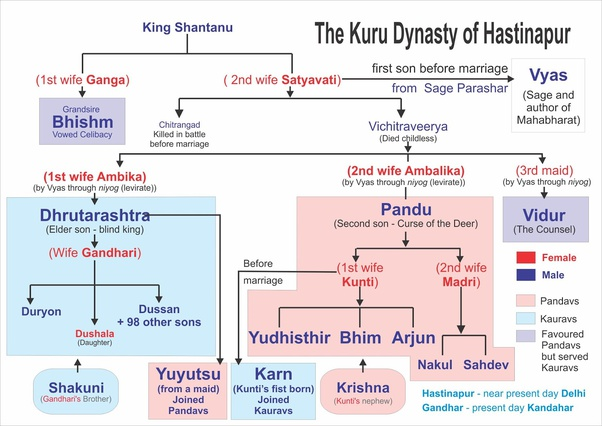
\includegraphics[scale = 0.75]{image3.png}\footnote{"Mahabharata
  - Ancient History Encyclopedia." Accessed October 21, 2020.
  \href{https://www.ancient.eu/Mahabharata/}{\underline{https://www.ancient.eu/Mahabharata/}}.}

\end{center}

\subsection{Map}
\begin{center}

\includegraphics[scale = 1]{image1.png}\footnote{"Map
  of India during Ramayana and Mahabharata -- तमसो ...." Accessed
  October 29, 2020.
  \href{https://vibhanshu.wordpress.com/2009/01/13/map-of-india-during-ramayana-and-mahabharata/}{\underline{https://vibhanshu.wordpress.com/2009/01/13/map-of-india-during-ramayana-and-mahabharata/}}.}
\end{center}

\newpage
\section{Committee Background}
\subsection{History of Mahabharata}

Mahabharata is a
\texttt{\underline{\href{https://drive.google.com/file/d/1tnbVYD9NxvcBGNo234wo7V1erBmfM39e/view?usp=sharing}{\textbf{Sanskrit}}
(sun-skrith)}} word meaning ``The Great Epic of the
\texttt{\underline{\href{https://drive.google.com/file/d/1CM2SWn9Ga6b8EJJHPf9uSBCQ5e5R3w-B/view?usp=sharing}{\textbf{Bharata}}
(baa-ruth)}} Dynasty''. It is one of the two major epics to detail the
ancient history of India, with the other being the
\texttt{\underline{\href{https://drive.google.com/file/d/1Z0gwiwo5oJ2E381tErtuf8x_P8xo12LC/view?usp=sharing}{\textbf{Ramayana}}
(raa-mai-yuhn)}}. The Mahabharata comprises 74,000 verses and 100,000
couplets, making the work a staggering 1.8 million words in total. This
makes it the longest epic poem in the world, and it is ten times the
length of the \emph{Iliad} and the \emph{Odyssey} combined. Due to the
sheer length of the story, scholars have long tried to figure out when
the Mahabharata was completed in full, and have narrowed the time frame
to the third and fifth centuries C.E.\footnote{"Mahabharata - New World
  Encyclopedia." Accessed October 21, 2020.
  \href{https://www.newworldencyclopedia.org/entry/Mahabharata}{\underline{https://www.newworldencyclopedia.org/entry/Mahabharata}}.}
The story, however, is widely considered by Hindus to be a chronicle of
history and the development of Hinduism from 400 B.C.E. to 200 C.E. This
is also attributed to the fact that the
\texttt{\underline{\href{https://drive.google.com/file/d/1dDCchIaspH3Gc2X0PsDk8tKNUr-pomEB/view?usp=sharing}{\textbf{Bhagavad
Gita}} (bug-vuhd gee-tha)}}, one of the
\texttt{\underline{\href{https://drive.google.com/file/d/16l7bBvgQJhfYlYcDWtfayBRAAy1PLmzL/view?usp=sharing}{\textbf{Hindu}}
(hin-doo)}} holy texts, is a part of the Mahabharata.\footnote{"Mahabharata
   Definition, Story, History, \& Facts
  Britannica." Accessed October 21, 2020.
  \href{https://www.britannica.com/topic/Mahabharata}{\underline{https://www.britannica.com/topic/Mahabharata}}.} \\

Although it has been theorized that more than one person wrote the epic,
authorship is usually conferred to the sage
\texttt{\underline{\textbf{\href{https://drive.google.com/file/d/12cpmbRkjohkLqUEyaP0_y7Y2CXE5YVam/view?usp=sharing}{Vyas}}
(vi-yas)}}. Due to the veracity of the Mahabharata itself being disputed,
scholars are unsure as to when Vyas lived. However, certain facts about
Vyas' life are known and have been recorded. Vyas was born to
\texttt{\underline{\href{https://drive.google.com/file/d/1N6ZbkjVOR-5Tl6Nwk2oZ76M9zSoGGIcI/view?usp=sharing}{\textbf{Satyavati}}
(sath-yuh-vuh-thee)}} and
\texttt{\underline{\href{https://drive.google.com/file/d/1M3Rknc2l6nV_ri-ZFsxkXIlV-g-udIMh/view?usp=sharing}{\textbf{Brahmin
Parashara}} (braah-man par-sha-rah)}}. His mother, Satyavati, was a
ferryman's daughter, and his father, the Brahmin, was a wandering sage
descended from
\texttt{\underline{\href{https://drive.google.com/file/d/1UBiNRUMQkQvRFdLQz8eNvUXrkh54ZBk0/view?usp=sharing}{\textbf{Vasistha}}
(vah-shisht)}}.\footnote{"Vyasa - New World Encyclopedia." Accessed
  October 21, 2020.
  \href{https://www.newworldencyclopedia.org/entry/Vyasa}{\underline{https://www.newworldencyclopedia.org/entry/Vyasa}}.}
Vasistha was one of the seven great
\texttt{\underline{\href{https://drive.google.com/file/d/1fETQfhYClXYbkn93U9efp-HwMDWboKcR/view?usp=sharing}{\textbf{Rishis}}
(ri-shees)}}, a yogi or an enlightened sage, during the
\texttt{\underline{\href{https://drive.google.com/file/d/18eL4_zTSc2jrYVD77qUzqoOmFkoZHqor/view?usp=sharing}{\textbf{Vedic}}
(vai-dik)}} times.\footnote{"Saptarishi and their contributions to the
  world - Vedicfeed." Accessed October 21, 2020.
  \href{https://vedicfeed.com/saptarishi-and-their-contributions/}{\underline{https://vedicfeed.com/saptarishi-and-their-contributions/}}.}
Vyas was born on an island covered in
\texttt{\underline{\href{https://drive.google.com/file/d/1VLNfXsKVPXZJmbgkvntV1IddTk5T7wZm/view?usp=sharing}{\textbf{Badara}}
(buh-daa-raa)}} trees (Indian Jujube trees), which earned him the name
\texttt{\underline{\href{https://drive.google.com/file/d/1F2arjRC_vmOMQkIiy4Kb1HUtYKybG49q/view?usp=sharing}{\textbf{Dwaipayana}}
(dvai-pah-yaan)}}, which means ``island-born''. He was also born with
extremely dark skin, which is why he was also called
\texttt{\underline{\href{https://drive.google.com/file/d/1e9kEn5cHUmHbHilre2HvLMAYKAPRULKg/view?usp=sharing}{\textbf{Krishna}}
(krish-naa)}}. Vyas was the first child born to his mother, Satyavati,
before her marriage to the
\texttt{\underline{\href{https://drive.google.com/file/d/1gFKrESPxHORwef_wMx6tkKcAnqWETUaQ/view?usp=sharing}{\textbf{Kuru}}
(koo-ru)}} King
\texttt{\underline{\href{https://drive.google.com/file/d/1k408zauSh2KHX84Dkm-jQeVLiv5DU9-6/view?usp=sharing}{\textbf{Shantanu}}
(shaan-tha-noo)}}, the king of
\texttt{\underline{\href{https://drive.google.com/file/d/17JxCzWzAyMEJIt51NBOgksl19dW2KkBN/view?usp=sharing}{\textbf{Hastinapur}}
(has-thee-naa-pur)}}.\footnote{Ibid} \\

King Shantanu was the youngest son of the Kuru King
\texttt{\underline{\href{https://drive.google.com/file/d/1cFMOXmljJqY1Ozkw8zhMyl3Y7uTlzg_3/view?usp=sharing}{\textbf{Pratipa}}
(praa-theep)}}, having earned the throne by default because all of his
older siblings forfeited their claim to the throne for varying reasons.
As king, Shantanu was walking the banks of the
\texttt{\underline{\href{https://drive.google.com/file/d/1lhsOVMsRz9JIYvKQYeOk1_5M4USAuRgc/view?usp=sharing}{\textbf{Ganga}}
(gun-gaa)}} river when one day he saw a beautiful mysterious woman. He
asked for the woman's hand in marriage and she agreed, but on one very
important condition. Shantanu could never question any actions by his
new wife, who unbeknownst to him, was the goddess Ganga (Hindu goddess
of the river). Once married, Ganga gave birth to her first son. After
the birth of her son, King Shantanu found Ganga drowning the child. Even
though he was upset, King Shantanu remembered the promise he had made to
his wife, and kept silent. However, this continued six more times, with
Ganga giving birth to seven sons total and drowning them all. Finally,
when the eighth son was born and Ganga went to drown him, King Shantanu
could no longer restrain himself. He confronted Ganga and asked how she
could kill their children and rob him of potential heirs. Ganga finally
revealed her identity to Shantanu and explained that she and her
children were the victim of a curse placed on her by
\texttt{\underline{\href{https://drive.google.com/file/d/1ZLRx23lThXknyJ40FbeLpn5CkJkJuviF/view?usp=sharing}{\textbf{Brahma}}
(bhra-maa)}}. Ganga explained that since Shantanu had broken the
condition in place by questioning her actions, she had to leave him, but
she wasn't going to kill their eighth child. Instead, Ganga took the
eighth son with the promise that she would return him to Shantanu in due
time.\footnote{"The story of Shantanu \textbar{} Mahabharata Stories,
  Summary and ...." Accessed October 21, 2020.
  \href{https://www.mahabharataonline.com/stories/mahabharata_character.php?id=45}{\underline{https://www.mahabharataonline.com/stories/mahabharata\_character.php?id=45}}.} \\

Eventually, a day came when King Shantanu was walking along the banks of
the Ganga river and noticed that the river had become extremely shallow.
Upon investigation, he discovered a young man standing in the river had
curbed the river's flow with a celestial weapon. The mysterious young
man recognized King Shantanu as his father, but instead of revealing
himself, instead disappeared using the power of illusion. King Shantanu
became frustrated and called upon the goddess Ganga to show herself and
explain who that young man was. Ganga appeared and introduced the man as
\texttt{\underline{\href{https://drive.google.com/file/d/1lthKwUjTzzscUKL2tPOHrR0aAlfg_nEK/view?usp=sharing}{\textbf{Devavrata}}
(dhe-vav-ruth)}}, the son of King Shantanu.\footnote{"Shantanu -- Vyasa
  Mahabharata." Accessed October 21, 2020.
  \href{https://www.vyasaonline.com/encyclopedia/shantanu/}{\underline{https://www.vyasaonline.com/encyclopedia/shantanu/}}.}
Devavrata had been taught political science by
\texttt{\underline{\href{https://drive.google.com/file/d/16Y6YUMikUEdmvmnieq0pjAi7FS8k6I7y/view?usp=sharing}{\textbf{Brihaspati}}
(brr-hus-puh-thee)}} (the guru of the Devas), knowledge of the
\texttt{\underline{\href{https://drive.google.com/file/d/1MTPm3EmU8PGgq2TPG95CLzbzy9gKVEDp/view?usp=sharing}{\textbf{Vedas}}
(vei-das)}} from Rishi Vasishta, and the art of archery from
\texttt{\underline{\href{https://drive.google.com/file/d/12Z_FvoFpsOF0ywvrrW5biNcu2Fkl8-qE/view?usp=sharing}{\textbf{Parashurama}}
(par-shur-um)}}. This had made Devavrata an exceptionally skilled
administrator, and an undefeatable warrior.\footnote{"The Story of
  Bhishma \textbar{} Mahabharata Stories, Summary and ...." Accessed
  October 21, 2020.
  \href{https://www.mahabharataonline.com/stories/mahabharata_character.php?id=44}{\underline{https://www.mahabharataonline.com/stories/mahabharata\_character.php?id=44}}.}
Devavrata promptly returned to Hastinapur with the king, where he was
crowned the heir. \\

Then King Shantanu met and fell in love with another woman, Satyavati,
who was the aforementioned mother of Vyas. Satyavati was the daughter of
\texttt{\underline{\href{https://drive.google.com/file/d/1po7hfZ6_t0pbceKlydD69WjDzy_lgTgU/view?usp=sharing}{\textbf{Dasharaj}}
(dhaash-raaj)}}, a fisherman and ferryman who raised Satyavati by the
\texttt{\underline{\href{https://drive.google.com/file/d/11iuj4w8FPec3wsC4q4F6-noLFrrQkqlT/view?usp=sharing}{\textbf{Yamuna}}
(yuh-moo-naa)}} river. When King Shantanu asked for Satyavati's hand in
marriage, Dasharaj refused.\footnote{"Satyavati -- Vyasa Mahabharata."
  Accessed October 21, 2020.
  \href{https://www.vyasaonline.com/encyclopedia/satyavati/}{\underline{https://www.vyasaonline.com/encyclopedia/satyavati/}}.}
He said that Satyavati's marriage to the King could only happen if it
was Satyavati's children that would have a claim to the throne. This
directly conflicted with King Shantanu's promise to Devavrata. In order
to please his father, Devavrata renounced his title as crown-prince.
This didn't fully please Dasharaj, who countered that Devavrata's
children could still claim the throne. Devavrata then vowed he would be
celibate for the rest of his life so that he wouldn't ever have any
offspring. This earned Devavrata the name of
\texttt{\underline{\href{https://drive.google.com/file/d/1dqqnqVBxGQG9JxwZKFaLFkW1fR3UFZah/view?usp=sharing}{\textbf{Bhishma}}
(bhee-shum)}}, which means ``he of the terrible oath''. This selflessness
and strictness of the oath taken by Bhishma earned him recognition by
the gods and his father, and he was granted the boon (blessing) of
\texttt{\underline{\href{https://drive.google.com/file/d/1yNX--rYMGQvSF9YZfBRnt9ztgANpzUjQ/view?usp=sharing}{\textbf{Iccha
Mrityu}} (itch-cha mri-thyu)}}. This boon stipulated that Bhishma could
choose the time of his death, but he was not immortal.\footnote{Ibid}
Thus Bhishma pledged eternal loyalty to defend whoever was on the throne
of Hastinapur. \\

King Shantanu and Satyavati had two sons together, named
\texttt{\underline{\href{https://drive.google.com/file/d/1ZE4rzdRU4OGeMofDFrix5tO9c8AlmrqB/view?usp=sharing}{\textbf{Vichitravirya}}
(vi-chit-ruh-veer-yuh)}} and
\texttt{\underline{\href{https://drive.google.com/file/d/13KRNPmCrKWRmb9dF9hgtAD0gQqaVsn4l/view?usp=sharing}{\textbf{Chitrangada}}
(chit-raang-daa)}}. When King Shantanu passed away, he passed the throne
to Vichitravirya. Both of King Shantanu's sons died childless, and
Satyavati arranged for more heirs to be produced using the ancient
practice of
\texttt{\underline{\href{https://drive.google.com/file/d/1mzZ2rCXC8DK4eaNB586vkcrfG5IlpvC3/view?usp=sharing}{\textbf{Niyoga}}
(nee-yogh)}}. Niyoga is when another man can father children with the
widow whose husband dies childless. Satyavati requested that Vyas
produce sons with both of Vichitravirya's widows, named
\texttt{\underline{\href{https://drive.google.com/file/d/1WC1iP0uX5S0hR5Az2hL8e8EoiWK_QMH4/view?usp=sharing}{\textbf{Ambika}}
(um-beek-ah)}} and
\texttt{\underline{\href{https://drive.google.com/file/d/18X8b4SJRXKLsA0hl72osL-HCopTfo_eQ/view?usp=sharing}{\textbf{Ambalika}}
(um-ba-leek-ah)}}. When Ambika was sent to Vyas, it is said that she
closed her eyes out of shyness and her aversion to Vyas' appearance.
Because of this, Vyas told Satyavati that Ambika's son
\texttt{\underline{\href{https://drive.google.com/file/d/1GMnpGiv2kfdLG2qlgDb0rvvrhwiAxwIf/view?usp=sharing}{\textbf{Dhritarashtra}}
(dri-tharash-thruh)}} would be born blind, and therefore would be unfit
to rule. Satyavati then warned Ambalika to remain calm when she saw
Vyas, but Ambalika grew pale when she saw him. Then, Vyas proclaimed
that Ambalika's son
\texttt{\underline{\href{https://drive.google.com/file/d/1aFWNBQKaua-edsIzc3RcmaoEFGVQs0Td/view?usp=sharing}{\textbf{Pandu}}
(paan-du)}} would be born anemic and also unfit to rule the kingdom.
Finally, Vyas asked for one of the wives to be sent to him again so that
they could produce a healthy heir. Instead, Ambika and Ambalika sent one
of the maids to see Vyas. Due to the maid's calm and collected composure
upon seeing Vyas, he blessed her with a healthy baby named
\texttt{\underline{\href{https://drive.google.com/file/d/1NhyX-PaApdpWOtrL1TMxd2-TPazUcA8v/view?usp=sharing}{\textbf{Vidura}}
(vi-dur)}}.\footnote{Ibid} \\

\newpage
\subsection{History of the Kauravas \texttt{\href{https://drive.google.com/file/d/1ptzaOxqQtvT8BU7IC_lnXLczsqRelJKU/view?usp=sharing}{
(kau-ruhvs)}}}

\begin{wrapfigure} {r} {0.4\linewidth}
\centering

\includegraphics[scale = 0.6]{image5.png}
\end{wrapfigure}

Since Pandu could not become king due to the curse placed on him by
Rishi
\texttt{\underline{\href{https://drive.google.com/file/d/1wyiIggoZmhyi-JTpN7m8qYUUnm89fVhN/view?usp=sharing}{\textbf{Kindama}}
(kin-dham)}}, Dhritarashtra, Pandu's brother, was given the throne.
However, Dhristarashta had been blind from birth. Nonetheless, he was no
less than Pandu in any way. He had received the same military training
and education as Pandu. Dhristarashta married
\texttt{\underline{\href{https://drive.google.com/file/d/1a35me9JQc6RU3jx1ZZiAjeBDBq_GsP5X/view?usp=sharing}{\textbf{Gandhari}}
(ghaan-dhaa-ree)}}, who decided that like her husband, she too would live
in darkness. Gandhari covered her eyes by tying a silk cloth. She
declared that she would only open the tie upon her
death.\footnote{"Mahabharata - Ancient History Encyclopedia." Accessed
  October 21, 2020.
  \href{https://www.ancient.eu/Mahabharata/}{\underline{https://www.ancient.eu/Mahabharata/}}.}

While Gandhari was queen of Hastinapur, a famous sage, Dwaipayana, came
to visit the palace. Gandhari personally looked after the comforts and
needs of the sage. Dwaupayana was so impressed by her care and her
selfness that he granted her a boon. Gandhari asked for a 100 sons that
would equal her husband in accomplishments. Dwaipayana granted her wish,
and Gandhari became pregnant.\footnote{"Kauravas - Ancient History
  Encyclopedia." Accessed October 21, 2020.
  \href{https://www.ancient.eu/Kauravas/}{\underline{https://www.ancient.eu/Kauravas/}}.} \\

Two years later, Gandhari was still pregnant. She showed no signs of
delivering anytime soon. At the same time,
\texttt{\underline{\href{https://drive.google.com/file/d/1_UA258lmi4N9VQho4kpciVNRPHq_zYGq/view?usp=sharing}{\textbf{Kunti}}
(kun-thee)}}, Pandu's wife, had birthed five divine sons. Hearing of the
birth of Kunti's sons, Dhritrashtra was furious at them being born first
because the oldest son is always favored for the throne of Hastinapur.
Meanwhile, Gandhari also became infuriated with her everlasting
pregnancy, and she hit her abdomen hard.\footnote{Ibid} Soon after
instead of delivering a baby, Gandhari delivered a horrifying lump of
mass. Upset and dejected, Gandhari went to look for Sage Dwaipayana. She
complained to Dwaipayana and doubted the sincerity of his boon. The sage
replied that he had never lied, not even in jest. She would have her 100
sons.\footnote{Ibid} \\

Dwaipayana told Gandhari to go back and cut her lump of mass into a 100
pieces. Gandhari cut the mass of lump into 101 pieces because she also
wanted a daughter. She placed each piece into a separate pot and filled
each pot with ghee, or clarified butter. Finally Gandhari's wish was
granted and the first Kaurava,
\texttt{\underline{\href{https://drive.google.com/file/d/1nwSSBrQIJ-UQO-p-WC-Bg4Z1qNjTfhZM/view?usp=sharing}{\textbf{Duryodhana}}
(dur-yo-dhan)}}, was born. When he was born, several animals started
howling nonstop. This was considered a bad omen, and Vidura advised
Dhritarashtra and Gandhari to drown the child in the holy river Ganga.
Both parents refused to give up their first child, and this decision
would very much shape their future. Duryodhana's birth was soon followed
by his 99 brothers, and his sister,
\texttt{\underline{\href{https://drive.google.com/file/d/1Gkniqa3c5mc059Q6FvZy0ePza_KB-ley/view?usp=sharing}{\textbf{Dussala}}
(dhoo-sha-laa)}}.\footnote{"Mahabharata - Ancient History Encyclopedia."
  Accessed October 21, 2020.
  \href{https://www.ancient.eu/Mahabharata/}{\underline{https://www.ancient.eu/Mahabharata/}}.} \\

The Kauravas' childhood was full of love and care. All 101 siblings were
doted on by both their parents. The Kauravas got their education and
military training from
\texttt{{\href{https://drive.google.com/file/d/1GKVU-TaPGP4vNyE8pDSzUfNHyKCW4HNQ/view?usp=sharing}{\textbf{Guru
Dronacharya's (Drona)}} (goo-ru droh-naa-chaar-yuh) (droh-naa)}}, who
also taught the
\texttt{\underline{\href{https://drive.google.com/file/d/1Y0e1yo3w49t4CobFlTryZT7ixmMI-Afd/view?usp=sharing}{\textbf{Pandavas}}
(pahn-duhvs)}}.\footnote{Ibid} Additionally, Duryodhana was given the
opportunity to learn mace fighting from
\texttt{\underline{\href{https://drive.google.com/file/d/1L1LAcxF9GZlhvnOF1qFWHk4IXZza3IzJ/view?usp=sharing}{\textbf{Balarama}}
(bah-laa-raam)}}, an older brother of Lord Krishna. Balarama also taught
mace fighting to
\texttt{\underline{\href{https://drive.google.com/file/d/1dqTu2tLHafrNZbKqC5MUVBXEptNpt2K7/view?usp=sharing}{\textbf{Bhima}}
(bhee-muh)}}, a Pandava. Both Duryodhana and Bhima were the best students
and extremely talented at their respective fighting styles.\footnote{"Kauravas
  - Ancient History Encyclopedia." Accessed October 20, 2020.
  \href{https://www.ancient.eu/Kauravas/}{\underline{https://www.ancient.eu/Kauravas/}}.} \\

The Kauravas harbored a large resentment toward the Pandavas. They
developed a hatred for the Pandavas early on because of the lineage to
the royal throne. Duryodhana was especially jealous and hateful towards
Bhima. Bhima was younger than Duryodhana, yet he was faster and
stronger. The Kauravas blamed the Pandavas for being ambitious and
wanting to steal the throne of Hanstinapur from them, the rightful
heirs. They believed it should be Duryodhana who should be crowned king
as the eldest of the Kaurava sons.\footnote{Doniger, Wendy. n.d.
  ``Mahabharata.'' Britannicia. Accessed October 20, 2020.
  \href{https://www.britannica.com/topic/Mahabharata}{\underline{https://www.britannica.com/topic/Mahabharata}}.} \\

During the Kauravas' childhood,
\texttt{\underline{\href{https://drive.google.com/file/d/1W6-9A5tCvrCfKQBv-zHQ1JtPp9EI0-eM/view?usp=sharing}{\textbf{Shakuni}}
(sha-ku-nee)}}, Gandhari's brother, intentionally fed into the Kaurava
children's righteousness. Shakuni pledged to make a Kaurava son the
rightful King of Hastinapur.\footnote{Ibid} He encouraged Duryodhana's
narcissistic pride. The hate between Kauravas and Pandavas that started
during childhood and festered throughout their lives would set the stage
for an epic battle. \\


\subsection{History of the Pandavas}

The Pandavas are the offspring of Pandu----the grandson of King
Shantanu, nephew of Bhishma, and brother of Dhritarashtra. He was
crowned King of Hastinapur because his brother, Dhritarashtra, was
blind. Pandu had two wives: Kunti and Madri. \\

\begin{wrapfigure} {r} {0.5\linewidth}
\centering
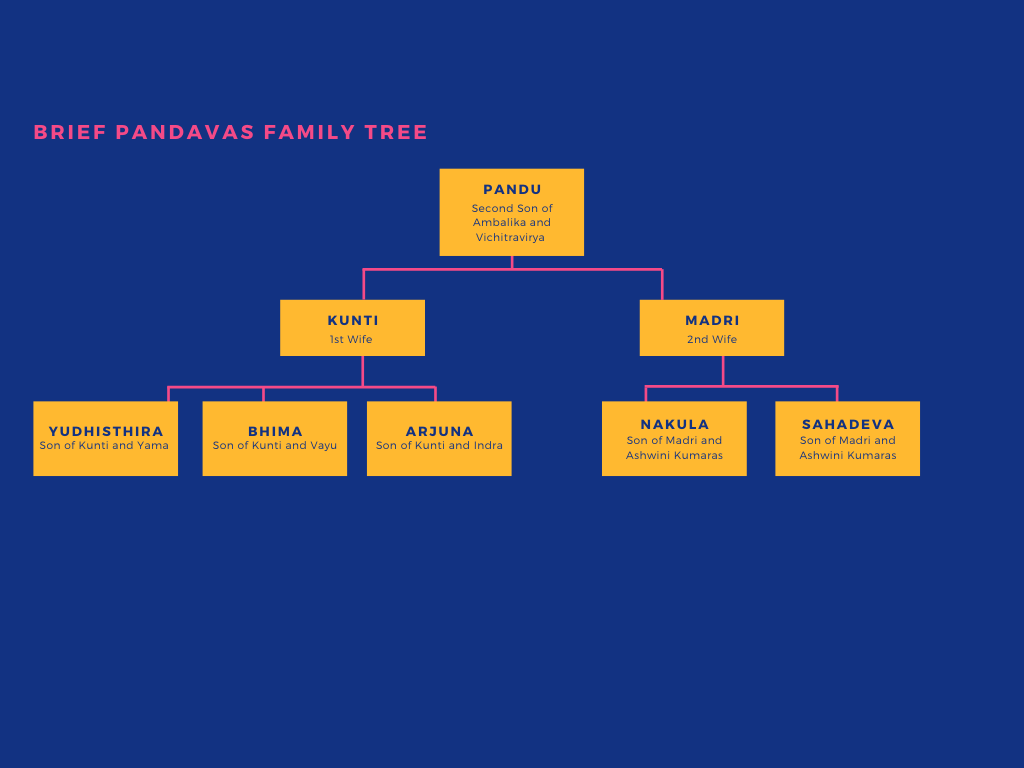
\includegraphics[scale = 0.25]{image2.png}
\caption{A short Pandava family tree}
\end{wrapfigure}

While hunting one day in the forest, Pandu saw a pair of deer
fornicating, so he shot them with arrows. The deer turned out to be the
sage Rishi Kindama and his wife making love in the form of deer. As the
sage (a profoundly wise man often in legend and mythology) lay dying, he
placed a curse on Pandu because Pandu had not only killed him and his
wife while they were making love, but Pandu was also not remorseful for
his actions. The curse stipulated that Pandu would die if he ever
approached either of his wives with the intention of having intimate
relations.\footnote{"Pandavas - Ancient History Encyclopedia." Accessed
  October 20, 2020.
  \href{https://www.ancient.eu/Pandavas/}{\underline{https://www.ancient.eu/Pandavas/}}.}
With knowledge that his actions were wrong and that he could no longer
produce heirs to the throne, Pandu abdicated the throne of Hastinapur.
Thus, Dhritarashtra, the blind son, became King of Hastinapur. \\

Due to the curse, Pandu could not engage in sexual intercouse with any
of his wives. However, Pandu's first wife Kunti was given a boon
(blessing) from another sage. The boon was that if she chanted a mantra,
she could invoke any god of her choice and get a son from him. Thus,
Pandu and Kunti got their first son,
\texttt{\underline{\href{https://drive.google.com/file/d/1dHaDih0_FCGK9IaZ9dmPu9QiL1iJIu2U/view?usp=sharing}{\textbf{Yudhishthira}}
(yood-his-thir)}}, from the god of death
\texttt{\underline{\href{https://drive.google.com/file/d/1La94GsbuOIy-rix4BHMg0Tzy2OBtlPXC/view?usp=sharing}{\textbf{Yama}}
(yaam)}}. Their second son, Bhima, was a gift from the god of wind
\texttt{\underline{\href{https://drive.google.com/file/d/168kEEnStpOVtdu9epuk19b5McRbLB53-/view?usp=sharing}{\textbf{Vayu}}
(vaa-yu)}}, and their third son,
\texttt{\underline{\href{https://drive.google.com/file/d/1OymnP6tbvSLX3VR0o16n-NMKHkrhL8qt/view?usp=sharing}{\textbf{Arjuna}}
(ar-joon)}}, was from the king of heaven
\texttt{\underline{\href{https://drive.google.com/file/d/1lUnkqGozjpFi9nhVtd4Biq3SyFwb3o4g/view?usp=sharing}{\textbf{Indra}}
(indh-ruh)}}. After having their three sons, Kunti transferred her boon
to Pandu's second wife,
\texttt{\underline{\href{https://drive.google.com/file/d/1pMTyMAA9wdBqE6WSLOLpjUGlxoaEGpwF/view?usp=sharing}{\textbf{Madri}}
(maa-dhree)}}. Madri then had two more
sons----\texttt{\underline{\href{https://drive.google.com/file/d/1u-QMw8C7J2NHIyzaA-0XnRQ6t3Qsihaq/view?usp=sharing}{\textbf{Nakula}}
(naa-kul)}} and
\texttt{\underline{\href{https://drive.google.com/file/d/1lvmEuwtmY9J6ANDS-rBD4-8ZyXIqjKH0/view?usp=sharing}{\textbf{Sahadeva}}
(suh-huh-dev)}}----from the
\texttt{\underline{\href{https://drive.google.com/file/d/1zBC2Yhh5JPbpFRagdS72vNfFWh1ug4VC/view?usp=sharing}{\textbf{Ashwini
Kumaras}} (ash-vi-nee kum-ars)}}, the Hindu Vedic gods of medicine. All
of the Pandava sons were born in the forest where Pandu and his wives
were in exile.\footnote{Ibid} \\

\subsection{The Death of Pandu}

One day, Pandu forgot about the curse and made love to Madri.
Afterwards, the curse was fulfilled, and Pandu died. In grief, Madri
committed sucide, and Kunti adopted her sons. Following Madri and
Pandu's demise, Kunti took all five sons back to Hastinapur.\footnote{``Birth
  of Pandavas and Kauravas.'' n.d. Hinduism for Kids. Accessed October
  20, 2020. \\

  \href{https://www.hindujagruti.org/hinduism-for-kids/589_birth-of-pandavas-kauravas.html}{\underline{https://www.hindujagruti.org/hinduism-for-kids/589\_birth-of-pandavas-kauravas.html}}.}
Upon return, Dhritarashtra named Yudhishthira the crown-prince much to
the chagrin of Dhritarashtra's eldest son, Duryodhana. While in
Hastinapur, the Pandavas also met their cousins, the Kauravas. The
Kauravas kept taunting the Pandavas, and the cousins got into many
disagreements. All of the Pandava sons were sent to Guru Drona's school
to train in advanced military arts as decided by their grandfather,
Bhishma. Arjun trained in archery, Bhima in mace fighting, and so on.
When Drona had deemed their training appropriate, he arranged
tournaments for them to test their skills. No one was able to match
Arjuna's archery skills. A commoner,
\texttt{\underline{\href{https://drive.google.com/file/d/14PQrVcz19KHFIB80ZpAH2TP48Swfv1Qx/view?usp=sharing}{\textbf{Karna}}
(kuhrn)}}, appeared and demanded a battle with Arjuna. Karna was insulted
by Bhima for being of mixed caste. This sparked the beginning of a feud
between the Pandavas and Karna. Duryodhana became friends with Karna by
giving him some territory from the Kuru empire so he would be considered
a royal, so he could challenge Arjuna. This act cemented a friendship
between Karna and Duryodhana. \\

Once the brothers returned to Hastinapur, the Pandavas and their mother,
Kunti, lived in the \textit{Lakshagriha}
\texttt{\underline{\href{https://drive.google.com/file/d/1O2Fe5xmf1yizyU5i_9_czAq1LKjG-Mgf/view?usp=sharing}{
(laak-shaa-gri)}}} (House of Wax) in the forest of
\texttt{\underline{\href{https://drive.google.com/file/d/1Wyu7hZoFD6tMbyiD59ENtRi3iI0UJVVA/view?usp=sharing}{\textbf{Varnavat}}
(var-naa-vuth)}}. The plan to build the \emph{Lakshagriha} was Duryodhana
and Shakuni's. It was meant to be a death trap as wax is highly
flammable, and no one would suspect foul play thus ruling the Pandavas'
death an accident. However, the Pandavas' uncle, Vidura, learned of the
plot and warned the Pandavas in time. Ultimately, the Pandavas were able
to escape safely. News of the fire at \emph{Lakshagriha} reached
Hastinapur, but Vidura was the only one that knew that the Pandavas were
safe. As a result, Duryodhana thought the Pandavas were dead. Vidura
shared with Bhishma that the Pandavas were indeed safe.\footnote{``Escape
  from Lakshagriha.'' n.d. Hinduism for Kids. Accessed October 20, 2020.
  ``Birth of Pandavas and Kauravas.'' n.d. Hinduism for Kids. Accessed
  October 20, 2020.
  \href{https://www.hindujagruti.org/hinduism-for-kids/589_birth-of-pandavas-kauravas.html}{\underline{https://www.hindujagruti.org/hinduism-for-kids/589\_birth-of-pandavas-kauravas.html}}.} \\

\subsection{The Hiding Period}

Kunti and the Pandavas lived in hiding after they escaped the murder
plot because Kunti believed that this would avoid further problems with
the Kauravas. The Pandavas took shelter in a forest and disguised
themselves as sages. The most important thing that happened during their
hiding period was the Pandavas meeting with Krishna, their maternal
cousin from Kunti's side. The Pandavas learned of a
\texttt{\underline{\href{https://drive.google.com/file/d/1LqbjDj6XmSM0e6Dyczf_hlx1PbWlZvaz/view?usp=sharing}{\emph{\textbf{swayamvara}}}
(svah-yum-vaar)}}, which was the practice of choosing a husband from a
list of eligible suitors, taking place for the hand of the
\texttt{\underline{\href{https://drive.google.com/file/d/1b7BXHC6ILJ7fihWaZi2QrmjnxZ-L9DzW/view?usp=sharing}{\textbf{Panchala}}
(paan-chaal)}} princess
\texttt{\underline{\href{https://drive.google.com/file/d/1poLMqFJ6fA-zwtX8SJnOBjxyjH_-FblM/view?usp=sharing}{\textbf{Draupadi}}
(drau-pah-dhee)}}. The Pandavas disguised themselves as Brahmins in order
to witness the event. Krishna befriended Draupadi, and he told her to
look out for Arjuna. The task to win Draupadi's hand was to string a
steel bow and shoot a target on the ceiling----the eye of a moving
artificial fish----while only looking at its reflection in the oil
below. Only three men present were reasonably capable of accomplishing
the task: Krishna, Arjuna, and Karna. Krishna was a spectator and a
friend of Draupadi, so he did not attempt the task. Karna was denied the
chance to compete by Draupadi given his low-born caste. When no royal
princes could successfully accomplish the task, the \emph{swayamvara}
was opened up to the Brahmins. Arjuna, who was disguised as a Brahmin,
won quite easily and went home after marrying Draupadi. When the
Pandavas got home, they said, ``Mother, see what we have brought today''
indicating Arjuna bringing back Draupadi. Without looking up, Kunti
said, ``Whatever it is, share it among yourselves.'' Aghast, they said,
``Mother, it's a woman. We have brought a princess.'' She turned around,
looked at Draupadi, the most stunning woman she had ever seen, and said,
``It doesn't matter. I told you to share, and that's it.''\footnote{Sadhguru.
  ``Mahabharat: Living the Story.'' \emph{Isha},
  \href{https://isha.sadhguru.org/us/en/wisdom/article/mahabharat-living-story}{\underline{https://isha.sadhguru.org/us/en/wisdom/article/mahabharat-living-story}}.} \\

Thus, Draupadi ended up becoming the wife of all five Pandava brothers.
She shared a bed with each brother for a year and rotated from there on.
Her opinion was regarded highly by all the five Pandava brothers, and
she was very intelligent. After the wedding, the Pandavas decided it was
time to go back to Hastinapur and claim what was theirs. The Kuru family
elders and relatives negotiated a split of the kingdom. The Pandavas
obtained a territory called
\texttt{\underline{\href{https://drive.google.com/file/d/1zOPec1WNyEgVvv7j8Q4BpgGtgPoxvOKR/view?usp=sharing}{\textbf{Khandavprastha}}
(khand-hav-prsth)}} which was filled with wild forests inhabited by Lord
\texttt{\underline{\href{https://drive.google.com/file/d/1I-daWDkgFOY-Yhs4YTtqHCRclkZYcSVA/view?usp=sharing}{\textbf{Takshaka}}
(thak-shak)}}, the King of Snakes and his family. Through hard work and
the help of Krishna, the Pandavas were able to rebuild the whole region,
including a new palace for themselves, and named it
\texttt{\underline{\href{https://drive.google.com/file/d/1wuEyqrnttfqtnH2HgrtRxoVmpSKUAIaw/view?usp=sharing}{\textbf{Indraprastha}}
(indruh-prasth)}}. They then invited their Kaurava cousins to their new
kingdom. As Duryodhana explored the palace, he did not see a crystal
screen and walked into it. As if that was not embarrassment enough, he
then fell into a pool, thinking it was a solid floor. Draupadi, Bhima,
Arjuna, Nakula, Sahadeva, and their servants laughed at him. Duryodhana
was enraged by their insults and jealous of the newfound wealth of
Pandavas, so Duryodhana decided to plan his revenge.\footnote{Ibid} \\

\subsection{The New Pandava Land, Indraprastha}

The news of Draupadi's marriage to the Pandavas spread fast across the
lands, eventually reaching Hastinapur. The blind King Dhritasrashtra
ordered a feast in the honor of the marriage, and he made arrangements
for the kingdom of Hastinapur to welcome the Pandavas. The Pandavas were
given a royal welcome back to Hastinapur. Upon their arrival,
Dhritasrashta called the five Panadavas to the throne room. After
consulting with his advisors, he had come to the decision to split a
portion of the kingdom off for the Pandavas. The Pandavas agreed to the
split portion.\footnote{``Mahabharat Episode 26: A New Beginning for the
  Pandavas.'' 2017. Isha.
  \href{https://isha.sadhguru.org/us/en/wisdom/article/mahabharat-26-pandavas-beginning}{\underline{https://isha.sadhguru.org/us/en/wisdom/article/mahabharat-26-pandavas-beginning}}.}
When Dhritarashtra decided to split the kingdom, he gave the Pandavas
the portion with a haunted forest. This forest was ruled by Lord
Takshaka, the King of Snakes. Yudhishthira knew the defaults of the
kingdom he was given, yet he accepted without any arguments.
Yudhishthira was getting ready to leave with the Pandavas when Lord
Krishna intervened on his behalf. Lord Krishna demanded that along with
the land, the treasures of the kingdom such as gold, horses, cattle,
etc, should be divided between the Pandavas and Kauravas. The generous
conditions put forth by Lord Krishna were unexpected, and Dhritarashtra
approved the offer because he wanted the Kauravas to look like
benevolent and fair leaders despite the fact that the Kauravas had just
offered the Pandavas a piece of land overrun by snakes.\footnote{Ibid} \\

After the splitting of the kingdom, many people of Hastinapur decided to
go with the Pandavas. They started on the long trek to their new
kingdom. With the help of Lord Krisnha, the Pandavas were able to
successfully settle in their new kingdom of Indraprastha overnight. Lord
Krishna quickly built palaces, towers, and new buildings in an area that
was previously seen as uninhabitable. The Pandavas ruled their beautiful
kingdom very wisely. Yudhishthira was a just and fair king. The kingdom
flourished with peace and prosperity and the citizens were happy under
the Pandava rule. The news of this prosperity spread to Hastinapur where
Duryodhana was seething with jealousy and rage.\footnote{Anand, Gautam.
  2016. ``Chapter 17 -- Indraprastha : The New Pandava Land.''
  \href{https://mymahabharatblog.wordpress.com/2016/12/03/chapter-17-indraprastha-the-new-pandava-land/}{\underline{https://mymahabharatblog.wordpress.com/2016/12/03/chapter-17-indraprastha-the-new-pandava-land/}}.} \\

\newpage
\section{Starting Scenario: The Dice Game}

Due to his humiliation at Indraprastha and the continued successes of
Yudhishthira as a ruler, Duryodhana found himself growing increasingly
envious. For this reason, Duryodhana and his uncle Shakuni hatched up a
plan in which they could trick Yudhishthira into gambling away his
riches and kingdom. Shakuni knew he would win at the game of dice they
had planned due to his sheer skill at the game and his knowledge that
Yudhishthira would never turn down an opportunity to play. The Pandavas
are invited to the Kuru court and Yudhishthira is challenged to the game
of dice. As predicted, he is unable to resist and ends up gambling away
his kingdom, riches, brothers, and even his wife Draupadi. Now that
Draupadi is considered the property of Duryodhana, he ordered that she
sit on his lap and also ordered Dushasana to disrobe her as
well.\footnote{"Duryodhana -- Vyasa Mahabharata." Accessed October 21,
  2020.
  \href{https://www.vyasaonline.com/encyclopedia/duryodhana/}{\underline{https://www.vyasaonline.com/encyclopedia/duryodhana/}}.}
Draupadi prayed to Krishna to save her, and Krishna granted her a
miracle. As Dushasana unraveled her sari, the length of cloth seemed to
be never-ending and eventually he had to stop due to
exhaustion.\footnote{"Draupadi -- Vyasa Mahabharata." Accessed October
  21, 2020.
  \href{https://www.vyasaonline.com/encyclopedia/draupadi/}{\underline{https://www.vyasaonline.com/encyclopedia/draupadi/}}.}
An enraged Draupadi tries to curse the Kuru court, but before she is
able to, Dhritarashtra and Gandhari intervene. They fear revenge for the
actions of their son by their allies and the gods, and so they return
all of Yudhishthira's losses back to him, as well as granting Draupadi
two wishes.\footnote{Ibid} \\

Then, Duryodhana and Shakuni order that the game be played again.
However, this time the conditions have changed. Shakuni says that if
Yudhishthira loses this game, then he and his brothers must spend 13
years in exile. Additionally, the 13th year must be spent in hiding, and
if they are found by the Kauravas, then the Pandavas will be forced to
go into exile for another 13 years. This is where our committee begins.
You are all in the court of the Kuru family in Hastinapur deciding how
to move forward with the dice game conditions set in front of you. Will
you play the game and face exile? Or will you change the course of
history by setting your own rules? \\

\newpage
\section{Characters}

\begin{enumerate}

\item
  
  \textbf{Bhishma:} The son of King Shantanu and Ganga (goddess of the
  river), Bhishma is one of the most powerful warriors to have served
  the Hastinapur throne. Not only is Bhishma a great warrior, but he is
  also extremely intelligent, having been trained in the art of
  leadership by many great Rishis. Due to his oath of celibacy, Bhishma
  is seen as a prime example of an officer bound to his duty due to
  diligence and selflessness.
  
\item
  
  \textbf{Vyas:} Vyas is the author and one of the most important
  characters in the Mahabharata. He lives in the forest near
  \texttt{\underline{\href{https://drive.google.com/file/d/1ctcl-Kifl3_FC-85r-w0dtUBqPwg7l3s/view?usp=sharing}{\textbf{Kurukshetra}}
  (ku-rook-shay-thrah)}} and is able to observe some events of the
  Mahabharata as they unfold. He is the grandfather to both the Pandavas
  and the Kauravas and serves as a spiritual guide to them throughout
  the story. Certain Hindu traditions also believe that Vyas is an
  avatar, or a physical manifestation, of the god Vishnu.\footnote{Ibid}
  
\item
  
  \textbf{Draupadi:} She is considered one of the most important women
  in the Mahabharata. Draupadi is the daughter of
  \texttt{\underline{\href{https://drive.google.com/file/d/1DRSKdG2iXMycN3Y0mPwXKNU_s1o2KvcY/view?usp=sharing}{\textbf{Draupada}}
  (drau-padh)}}, the King of Panchala. Draupadi is described as a
  beautiful dark-skinned woman, and upon her birth, it is prophesied
  that she would bring about the destruction of the Kuru line. She is
  the wife of each of the Pandava brothers and a good friend of the god
  Krishna.\footnote{Ibid}
  
\item
  
  \textbf{Vidura:} Meaning skilled, intelligent, or wise in Sanskrit,
  Vidura serves as the trusted advisor to King Dhritarashtra during his
  rule. By being the uncle of both clashing families and a half-brother
  to King Dhritarashtra and Pandu, he is a respected authority figure to
  the Pandavas as well, even going so far as to warn them about
  Duryodhana's plans to sabotage them.\footnote{"Vidura -- Vyasa
    Mahabharata." Accessed October 21, 2020.
    \href{http://www.vyasaonline.com/encyclopedia/vidura/}{\underline{http://www.vyasaonline.com/encyclopedia/vidura/}}.}
  
\item
  
  \textbf{Yudhishthira:} The firstborn son of Pandu and Kunti from Yama
  (the God of Death). As the firstborn son, he is the rightful heir
  according to the order of succession. He is the most truthful man to
  have ever lived, having never lied to anyone, or disobeyed anyone.
  
\item
  
  \textbf{Bhima:} The second son of Pandu and Kunti from Vayu (the God
  of Wind). Bhima is hotheaded, and always ready to fight. He is skilled
  in mace fighting, and he is one of the strongest people in the
  kingdom. Bhima also married a
  \texttt{\underline{\href{https://drive.google.com/file/d/1MvynrAayXduZipLCU3J3MlLGPRW-anp0/view?usp=sharing}{\textbf{Rakshasi}}
  (rak-sha-si)}}, a female demon.
  
\item
  
  \textbf{Arjuna:} The third son of Pandu and Kunti from Indru (the God
  of Heavens). Arjuna is the second-most skilled archer in the kingdom,
  after Karna. He is the closest to the five brothers' wife, Draupadi
  and her friend, Lord Krishna.
  
\item
  
  \textbf{Nakul:} The first twin born to Pandu and Madri, from Ashwini
  Kumaras (the Gods of Medicine). He is a skilled swordsman and is
  rumored to be one of the most handsome men in Hasanpur. Nukul is
  prominently talented in
  \texttt{\underline{\href{https://drive.google.com/file/d/1DBhFt8kpg8uhb4hOCWXNuWpg1fKumpgj/view?usp=sharing}{\textbf{Ayurveda}}
  (ai-yoor-veda)}}, which is the practice of traditional medicine.
  
\item
  
  \textbf{Sahdev:} He is the twin of Nukul, and the youngest Pandu.
  Sahdev is often overlooked as the last Pandu, however, he is very
  skilled in fighting, especially with an axe. He is also very skilled
  in Ayurveda.
  
\item
  
  \textbf{Kunti:} She is the mother of the three eldest brothers of the
  Pandavas; Kunti was given a boon with which she could call on any
  deity and have a child with him without pregnancy. She is the first
  wife of Pandu, and the sister of
  \texttt{\underline{\href{https://drive.google.com/file/d/139X4vOrEpzwGqjfrPLO7SG2t1NJjEgDf/view?usp=sharing}{\textbf{Vasudeva}}
  (va-su-dev)}}, the father of Lord Krishna. Kunti is a woman with high
  morals and social values, and she is always guiding her sons' actions.
  
\item
  
  \textbf{Karna:} Karna is the first son of Kunti, who used her mantra
  to summon
  \texttt{\underline{\href{https://drive.google.com/file/d/1fEW3QjbmhBje9W737N1ulmb1f17kCwT-/view?usp=sharing}{\textbf{Surya}}
  (soor-yuh)}}, the sun god, and have Karna. He was abandoned by Kunti
  but was soon taken in by King Dhritarashtra's charioteer,
  \underline{\href{https://drive.google.com/file/d/13Chs3HPXTn_XgPFZ06OKbUmUajkvxqVE/view?usp=sharing}{\textbf{Adhiratha}}
  (uh-dhi-rath)}. As Karna grows into adulthood, he becomes a warrior
  and seeks a position in the Hastinapur court by competing in a
  tournament, where he forms a strong bond with Duryodhana and a rivalry
  with his half-brother Arjuna.
  
\item
  
  \textbf{Duryodhana:} Duryodhana is the eldest Kaurav brother and the
  son of the blind King Dhritarashtra and Queen Gandhari. He is the
  crown-prince of the Kuru Kingdom and its capital Hastinapur along with
  his cousin Yudhishthira. He is loved by his family, but he has never
  been seen as equal to the Pandavas. Duryodhana is mentored by his
  uncle, Shakuni, who helps him mastermind plots against the Pandavas.
  
\item
  
  \textbf{Gandhari:} Gandhari is the princess of
 \texttt{ \underline{\href{https://drive.google.com/file/d/1z52DVt7sLKxwvSc1rVTklxelP2s2C3qw/view?usp=sharing}{\textbf{Gandhara}}
  (gaand-haar)}}, Shakuni's sister, and the wife of the blind King
  Dhritarashtra. She is also the mother of a hundred sons and one
  daughter, the Kauravas. Gandhari is a virtuous woman and has high
  morals. Unfortunately, most of Gandhari's sons do not hold the same
  values as her.
  
\item
  
  \textbf{Dhritarashtra:} Dhritarashtra is the blind son of the late
  King Shantanu who is ruling the Kuru Kingdom and its capital,
  Hastinapur. He is not able to wield any weapons due to his blindness
  but is strong enough to crush iron with his bare hands. Although
  Dhritarashtra is a fair and just ruler, he is constantly torn between
  following moral law and the love he has for his eldest son,
  Dhritarashtra. He often condones the actions of his son solely because
  of his affection for him.\footnote{"Dhritarashtra -- Vyasa
    Mahabharata." Accessed October 21, 2020.
    \href{https://www.vyasaonline.com/encyclopedia/dhritarashtra/}{\underline{https://www.vyasaonline.com/encyclopedia/dhritarashtra/}}.}
  
\item
  
  \textbf{Dushasana:} Dushasana is a Kaurava prince and is the second
  eldest son of King Dhritarashtra and Gandhari. Dushasana is devoted to
  his elder brother, Duryodhana. As a result, he is closely involved in
  his older brother's schemes against the Pandavas and is in the Kuru
  court's inner circle. However, Dushasana has an affinity for alcohol
  and is considered to be weak.
  
\end{enumerate}

\end{document}
